\section{Technische Umsetzung}
In diesem Kapitel wird die Umsetzung des modellierten Systementwurfs als prototypische Implementierung im Detail beschrieben. Es gibt einen Einblick in den Prozess der Konfiguration eines Blockchain Netzwerks, das mehrere Unternehmen umfasst. Dabei wird Eingangs auf die zugrunde liegende Architektur des Business Netzwerks bezug genommen. Aufbauend auf dem Fundament des Business Netzwerks werden Geschäftslogik und Berechtigungssystem erläutert.

\subsection{Business Netzwerk}
Als Basis des Blockchain Systems dient ein Hyperledger Fabric Netzwerk. Alle Dienste des Netzwerks werden in einer virtualisierten Umgebung bereitstellt. Dazu wird die Container Technologie von Docker\footnote{Docker basiert auf Linux Techniken wie \textit{Cgroups} und \textit{Namespaces}, um isolierte Umgebungen innerhalb eines Hostsystems bereitzustellen \citep{Bengel2008,Oeggl2019}.} verwendet. Zum einen bietet sich die Container Technologie zur Umsetzung eines Prototyps an, da sie sehr viel flexibler und leichtgewichtiger ist als die konventionelle Virtualisierung über Virtuelle Maschinen \citep{Ahmed2018}. Zum anderen sind die Basis Komponenten zum aufspannen eines Hyperledger Fabric Netzwerks bereits von der Linux Foundation als Container Abbild bereitgestellt, was die Realisierung des Prototypen signifikant beschleunigt. Im folgenden wird die technische Umsetzung eines Peer Knotens mittels Docker beispielhaft beschrieben. Die anderen Systemkomponenten (siehe Kapitel \ref{system-design-concept}) verhalten sich vom Aufbau her äquivalent zu einem Peer Knoten, sie sind lediglich unterschiedlich konfiguriert um verschiedene Aufgaben auszuführen. Die Netzwerke beider Unternehmen werden in diesem Fall auf der selben Maschine betrieben. In einem produktiven Umfeld würde jedes Unternehmen seine eigene Umgebung bereitstellen.

Das Prototyp Netzwerk umfasst zwei Organisationen: \textit{Org1} und \textit{Org2}. Das Unternehmen \textit{Org1} verwendet den Domänennamen \textit{org1.example.com}. Der \acf{msp} für \textit{Org1} wird als \textit{Org1MSP} bezeichnet. Das Unternehmen \textit{Org2} verwendet den Domänennamen \textit{org2.example.com}. Der \acf{msp} für \textit{Org2} heißt \textit{Org2MSP}.

\paragraph{Netzwerk Komponenten}$~~$\\
Das Hyperledger Fabric Netzwerk besteht insgesamt aus den folgenden Komponenten und Schnittstellen:

\begin{itemize}
    \item Zwei Peer Knoten für \textit{Org1}
    \begin{itemize}
        \item \textit{peer0.org1.example.com}
        \item \textit{peer1.org1.example.com}
    \end{itemize}
    \item Eine \ac{ca} für \textit{Org1} (\textit{ca.org1.example.com})
    \item Zwei Peer Knoten für \textit{Org2}
    \begin{itemize}
        \item \textit{peer0.org2.example.com}
        \item \textit{peer1.org2.example.com}
    \end{itemize}
    \item Eine \ac{ca} für \textit{Org2} (\textit{ca.org2.example.com})
    \item Ein einzelner Orderer Peer (\textit{orderer.example.com})
\end{itemize}

\noindent
Jede dieser Komponenten stellt einen Docker Container dar und ist auf Netzwerkebene über seinen Hostnamen ansprechbar. Die gesamte Netzwerkkommunikation ist über das \ac{tls}-Protokoll\footnote{\ac{tls} ist ein hybrides Verschlüsselungsprotokoll, um Datenübertragungen vor Angriffen zu schützen \citep{RFC5246}.} abgesichert. Aus diesem Grund müssen alle Zertifikate der \ac{ca} auf dem Hostsystem zur Verfügung stehen, damit eine Kommunikation mit dem Netzwerk stattfinden kann. Für Organisation \textit{Org1} ist ein Administrator User angelegt mit Namen \textit{Admin@org1.example.com}. Ebenfalls ist für Organisation \textit{Org2} ein Administrator User angelegt der \textit{Admin@org2.example.com} heißt. Zusätzlich zu den Administrator Usern der Organisationen ist die \ac{ca} mit einem Standard User konfiguriert. Der \ac{ca} User besitzt im gegensatz zu den Administrator Usern keine Berechtigungen, um Smart Contracts (Chaincode) auf Peers des Netzwerk zu installieren. Damit die Peer Administatoren sich mit dem Netzwerk verbinden können wird ein Verbindungsprofil benötigt. In diesem Verbindungsprofil werden alle Komponenten des Netzwerks definiert und die zugehörigen \ac{tls} Zertifikate hinterlegt (siehe Anhang \ref{lst:connection-profile}). Verbindungsprofil und die digitale Identität des Administrator Users, bestehend aus Zertifikat und privatem Schlüssel, bilden zusammen die sogenannte \textit{Business Network Card}. Hiermit kann sich der Administrator User über eine Hyperledger Fabric \ac{cli} mit dem Netzwerk verbinden und Befehle absetzen.

\begin{figure}[H]
	\centering
	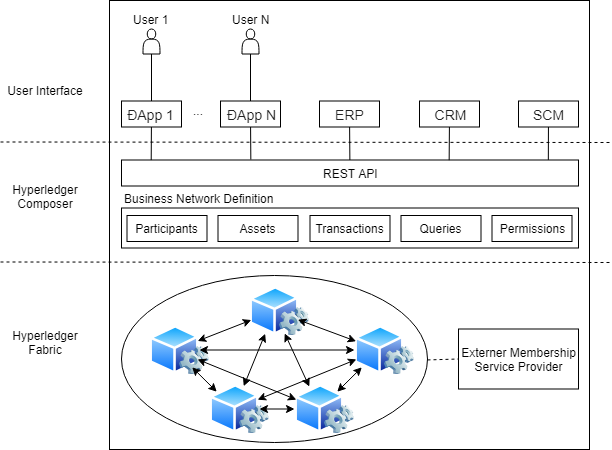
\includegraphics[width=1\linewidth]{pictures/poc-food-chain-traceability}
	\caption[Gesamtsystem Prototyp]{Gesamtsystem Prototyp}
	\label{fig:poc-food-chain-traceability}
\end{figure}

Nachdem starten der Docker Container lässt sich ein einfacher Smoke Test\footnote{Mit einem Smoke Test sollen grundlegende Probleme bei einer Software oder einem System offengelegt werden, bevor die Entwicklung von folge Komponenten begonnen wird \citep{Everett2007}.} durchführen, um sicherzustellen das das Netzwerk ordnungsgemäß hochgefahren wurde und alle Knoten arbeiten. Docker bietet zum Mangement der Container ein \ac{cli} an. Hiermit lässt sich der Smoke Test mit einem Einzeiler auf dem Terminal ausführen. Damit ist die Basiskonfiguration des Systems abgeschlossen und das Peer Netzwerk ist aufgespannt (siehe Abbildung \ref{fig:poc-food-chain-traceability} Abschnitt \textit{Hyperledger Fabric}). Im aktuellen Zustand kann das Netzwerk noch keine Transaktionen erzeugen oder verarbeiten. Dazu muss erst noch die im nächsten Kapitel beschriebene Geschäftslogik durch einen Administrator User auf einem Peer Knoten des Unternehmens installiert und instantiiert werden.

\subsection{Smart Contracts}
Smart Contracts heißen im Hyperledger Model \textit{Chaincode}. Sie setzen sich aus vier Elementen zusammen. Model, Logik, Zugriffskontrolle und Abfragedefinition bilden das sog. \acf{bna}. Das \ac{bna} lässt sich in jedes mit Hyperledger Fabric aufgespannte Blockchain Netzwerk deployen. Die Funktionsweise eines Smart Contracts soll hier am Beispiel des Eigentumswechsels eines Materials näher erläutert werden. Dazu wird auf jedes der vier Elemente eines \ac{bna} eingegangen, um den strukturellen Aufbau zu zeigen. Im Sinne des Models werden ein \textit{Participant}, ein \textit{Asset} und eine \textit{Transaction} mit einem \textit{Event} definiert wie in Listing \ref{lst:example-model-definition}. Die eigentliche Verarbeitungslogik wird gesondert von der Datenstruktur definiert (Listing \ref{lst:transaction-logic-change-ownership}). In diesem Fall wurde die Logik in der Programmiersprache JavaScript implementiert.

\begin{lstlisting}[caption={Model Example Definition},label=lst:example-model-definition]
namespace io.dev.foodchain

abstract participant Company identified by gln {
    o String gln
    o String name
}

participant Farmer extends Company {}

asset Material identified by materialId {
    o String materialId
    --> Company owner optional
}

transaction changeMaterialOwnership {
    --> Material material
    --> Company newOwner
}

event notification {
    --> Material changedMaterial
}
\end{lstlisting}

Zeile 1 in Listing \ref{lst:example-model-definition} definiert einen Namensraum für das gesamte Model. In einem produktiven Scenario würde ein Model erheblich größer sein, als das im Prototyp verwendete vereinfachte Model. Damit bei steigender Komplexität des abzubildenden Models Überblick und Wartbarkeit erhalten bleiben lässt sich das Model über mehrere Dateien abbilden und über den Namensraum auf logischer Ebene miteinander verknüpfen. Zeile 3 bis einschließlich Zeile 6 zeigt die Definition der abstrakten Klasse \textit{Company} vom Typ \textit{Participant}. Diese Definition wird in Zeile 10 konkret ausgeprägt durch die Klasse \textit{Farmer}. Äquivalent dazu werden auch alle anderen Teilnehmer der Wertschöpfungskette implementiert. Zeile 10 bis Zeile 14 zeigt die Implementierung des Assets \textit{Material}. Über die Eigenschaft \textit{owner} (Zeile 12) wird ein \textit{Material} später immer einem eindeutigen Besitzer zugeordnet. Die Eigenschaft \textit{owner} wurde dabei als direkte Ressourcenverknüpfung implementiert. Eine Ressourcenverknüpfung im Hyperledger Model lässt sich mit einer Fremdschlüsselbeziehung in einem relationalen Datenbankschema vergleichen. Die Eigenschaft kann in diesem Fall nur Werte annehmen, die eine gültige Ausprägung der abstrakten Klasse \textit{Company} darstellen und damit auch allen konkreten Ausprägungen dieser Klasse.

Um das Beispiel einfach und verständlich zu halten wurden die Definitionen der \textit{Participants} und \textit{Assets} in verkürzter Form abgebildet. Das vollständige Prototypen Model befindet sich im Anhang \ref{lst:hlc-model-definition}. Eine \textit{Transaction} mit zugehörigem \textit{Event} ist in Zeile 15 bis 22 dargestellt. Die \textit{Transaction} definiert dabei zwei Parameter als Ressourcenverknüpfung. Es werden das Asset \textit{material} sowie der neue Eigentümer \textit{newOwner} benötigt. Das \textit{Event} definiert nur einen Parameter und zwar eine Ressourcenverknüpfung zum angepassten Asset \textit{changedMaterial}. Wird das Event emittiert kann der Empfänger über die Ressource alle Informationen des Vorgangs nachvollziehen. In angebundenen \ac{ui} Applikationen kann dann auf das Event entsprechend reagiert werden bzw. können Drittsysteme beispielsweise Workflowprozesse auslösen.

\begin{lstlisting}[caption={Transaction Processor Function \textit{changeMaterialOwnership(tx)}},language=ES6,label=lst:transaction-logic-change-ownership]
/**
* Change material ownership transaction
* @param {io.dev.foodchain.changeMaterialOwnership} tx
* @transaction
*/
async function changeMaterialOwnership(tx) {
    const oMaterial = tx.material;
    const oNewOwner = tx.newOwner;
    const oActualOwner = tx.material.owner;

    const oMaterialRegistry = await getAssetRegistry(NS + '.Material');
    const bMaterialExists = await oMaterialRegistry.exists(oMaterial.getIdentifier());
    if(!bMaterialExists) {
        throw new Error('Input material does not exist.');
    }
    if (oMaterial.owner !== getCurrentParticipant()) {
        throw new Error('You are not allowed to change asset.');
    }
    const oParticipantRegistry = await getParticipantRegistry(oNewOwner.getNamespace());
    const bNewOwnerExists = await oParticipantRegistry.exists(oNewOwner.getIdentifier());
    if(!bNewOwnerExists) {
        throw new Error('New owner does not exist.');
    }

    oMaterial.ownerHistory.push(oActualOwner);
    oMaterial.owner = oNewOwner;
    await oMaterialRegistry.update(oMaterial);

    const oNotification = getFactory().newEvent('io.dev.foodchain', 'notification');
    oNotification.changedMaterial = oMaterial.getIdentifier();
    emit(oNotification);
}
\end{lstlisting}

Damit ein \textit{Participant} Funktionen auf einem \textit{Asset} ausführen kann wurden im vorherigen Abschnitt \textit{Transactions} modelliert. Zu jeder \textit{Transaction} Definition im Modell gehört eine Logikimplementierung. Verknüpft wird die Modelldefinition mit der Implementierung über die Annotation \textit{@transaction}. Eine \textit{Transaction} Funktion hat als einzigen Parameter das \textit{Transaction} Objekt. Über dieses Objekt kann innerhalb der Funktion auf alle Werte der Transaktion zurückgegriffen werden. Für das Beispiel des Eigentumswechsel wurde eine Transaktion definiert, die zum einen das \textit{Material} beinhaltet und zum anderen eine Referenz auf den neuen Eigentümer (siehe Listing \ref{lst:example-model-definition} Zeile 16 f.). Der Aufbau einer \textit{Transaction} Funktion folgt stets dem Muster - Initialiseren der Eingabeparameter, Plausibilitätsprüfungen, Geschäftslogik und abschließend die optionale Event Emittierung. Das Initialisieren der Eingabewerte wurde von Zeile 8 bis Zeile 10 implementiert. Es werden alle benötigten Werte der Transaktion zu lokalen Variablen zugewiesen. Zeile 14 bis Zeile 28 deckt die Plausibilitätsprüfung ab, hier wird geprüft ob im Falle des Eigentumswechsels

\begin{itemize}
    \item das \textit{Material} im Netzwerk vorhanden ist,
    \item der Transaktionsemittent auch Besitzer des \textit{Materials} ist und
    \item ob der neue Eigentümer als \textit{Participant} im Netzwerk vorliegt.
\end{itemize}

Die eigentliche Geschäftslogik ist relativ simpel und von Zeile 31 bis 33 implementiert. Für eine spätere Rückverfolgung der Eigentumsverhältnisse wird der aktuelle Eigentümer zur Eigentümerhistorie (Eigenschaft \textit{ownerHistory}) hinzugefügt und der neue Eigentümer wird gesetzt. Danach müssen die Assetänderungen noch an das Systemregister übermittelt werden. Das Schlüsselwort \textit{await} wird verwendet, da es sich hier um einen asynchronen Aufruf handelt und in der Logik so eine Haltemarke gesetzt wird sodass auf das Ergebnis des Aufrufs gewartet wird bevor mit der weiteren Verarbeitung der Funktion fortgefahren wird. Sollten bis zu diesem Zeitpunkt keine Fehler in der Verarbeitung aufgetreten sein, wird ein \textit{Event} erzeugt, mit Daten gefüllt und emittiert.

Einfache Berechtigungsprüfungen wie in der Transaktionslogik lassen sich auch über die Zugriffskontrolle regeln. Hyperledger unterscheidet zwischen der Zugriffskontrolle für Ressourcen innerhalb des Netzwerks und der Zugriffskontrolle für Änderungen seitens der Netzwerkadministration. Um den Zugriff auf eine Ressource zu steuern wird eine Regel definiert wie in Listing \ref{lst:model-permissions}. Diese Regel sagt aus, dass sie für jeden \textit{Participant} und bei jeder Operation (Lesen, Anlegen, Ändern, Löschen) angewandt wird (Zeile 3/4). Sie gilt für alle Ressourcen aus dem Namensraum \textit{io.dev.foodchain.*} und als Bedingung wurde definiert, dass der Besitzer \textit{r.owner.getIdentifier()} der Ressource gleich dem aktuellen \textit{Participant} ist (Zeile 5/6). Ist diese Regel erfüllt wird die Operation erlaubt bzw. bei nicht erfüllen der Zugriff auf die Ressource verweigert. Es ist anzumerken, dass die Regeln in der Reihenfolge ausgewertet werden in der sie definiert sind und die erste Regel deren Bedingung erfüllt ist, bestimmt ob der Zugang gewährt oder verweigert wird. Sofern keine Regel angewandt werden kann wird der Zugriff standardmäßig verweigert.

\begin{lstlisting}[caption={Berechtigungsdefinition},label=lst:model-permissions]
rule OwnerHasFullAccessToTheirAssets {
    description: "Allow all participants full access to their assets"
    participant(p): "io.dev.foodchain.*"
    operation: ALL
    resource(r): "io.dev.foodchain.*"
    condition: (r.owner.getIdentifier() === p.getIdentifier())
    action: ALLOW
}
\end{lstlisting}

\noindent
Das letzte Element des \acf{bna} ist die Abfragedefinition. Hier können für die Verwendung innerhalb der Transaktionslogik oder direkter Anfragen über externe Anwendungen \acs{sql}-ähnliche Abfragen formuliert werden. Listing \ref{lst:model-example-query} zeigt eine einfache Abfrage, um alle Assets vom Typ \textit{Material} zu selektieren für die gilt, das die boolesche Eigenschaft \textit{bonus} den Wert \textit{wahr} hat und das die Eigenschaft \textit{type} gleich dem Parameter \textit{\_\$type} ist. Parameter die innerhalb einer Anfrage definiert werden über den Präfix \textit{\_\$} müssen beim Aufruf der Abfrage mit übergeben werden. Über den eindeutigen Namen \textit{selectBonusMaterials} lässt sich diese Abfrage direkt in der Transaktionslogik ausführen.

\begin{lstlisting}[caption={Abfragedefinition},label=lst:model-example-query]
    query selectBonusMaterials {
      description: "Select materials based on bonus condition"
      statement:
          SELECT io.dev.foodchain.Material
              WHERE (bonus == true)
              AND (type == _$type)
              ORDER BY [status ASC]
    }
\end{lstlisting}

\noindent
In der \textit{statement} Eigenschaft einer \textit{Query} können jeweils folgende Operatoren verwendet werden:

\begin{itemize}
    \item \textit{SELECT} ist ein obligatorischer Operator und definiert standardmäßig das Register und den Asset- oder Teilnehmertyp, der zurückgegeben werden soll.
    \item \textit{FROM} ist ein optionaler Operator, der ein anderes Register für die Abfrage festlegt.
    \item \textit{WHERE} ist ein optionaler Operator, der die Bedingung definiert, die auf die selektierten anzuwenden sind.
    \item \textit{AND} ist ein optionaler Operator, der zusätzliche Bedingungen definiert.
    \item \textit{OR} ist ein optionaler Operator, der alternative Bedingungen definiert.
    \item \textit{CONTAINS} ist ein optionaler Operator, der Bedingungen für Array-Werte definiert.
    \item \textit{ORDER BY} ist ein optionaler Operator, der die Sortierung der Ergebnisse definiert.
\end{itemize}

\noindent
Damit ist das \acf{bna} vollständig und kann in einem Hyperledger Fabric Netzwerk installiert und instantiiert werden. Ein Netzwerkadministrator kann anschließend \textit{Participants} erzeugen und mit der digitalen Identität verknüpfen. Der Netzwerkteilnehmer ist daraufhin in der Lage Transaktionen im Netzwerk abzusetzen, um mit dem Smart Contract zu interagieren und Geschäftsvorgänge entsprechend abzubilden.

\subsection{Schnittstelle}
Damit die Funktionalität des Blockchain Netzwerks in bestehende IT Landschaften integriert werden kann bietet Hyperledger die Möglichkeit einen Smart Contract in Form einer \acs{rest}\footnote{\acf{rest} steht für ein Programmierparadigma für verteilte Systeme. Dabei wird der Zustand einer Ressource nicht gesondert gespeichert (Session) sondern über den \ac{uri} codiert.} \acs{api} für externe Anwendungen freizugeben.

Mit dem Ansatz einer \ac{rest} \ac{api} wird die Idee einer programmiersprachen unabhängigen Schnittstelle realisiert. Nahezu jede moderne Programmiersprache ist in der Lage simple \ac{http} Anfragen zu formulieren, über das Internet abzusetzen und das Resultat auszuwerten. Dadurch kann eine breite Masse an \ac{ui} Technologien und Frameworks verwendet werden, um für den Endanwender entsprechende Applikationen zur Nutzung der Smart Contract Funktionalität zu implementieren. Ebenfalls sind externe Systeme wie beispielsweise \ac{erp}-Systeme über die \ac{rest} \ac{api} in der Lage mit dem Blockchain Netzwerk zu kommunizieren und Asset Operationen auszuführen.

Die \ac{rest} Schnittstelle wird dabei nach der \textit{OpenAPI} Spezifikation \citep[siehe][]{OAI2018} generiert und zur Verfügung gestellt. Bei der Generierung wird aus den Modelldefinitionen und der Transaktionslogik die Klassen- und Funktionsdokumentation extrahiert und in der Schnittstellendokumention dargestellt.

Wird die \ac{rest} Schnittstellen über den Hyperledger Composer REST Server ausgeliefert erhält man eine Übersicht aller \textit{Assets, Participants, Transactions \& Queries} die über den Smart Contract abgebildet worden sind. Abbildung \ref{fig:rest-api-explorer} zeigt einen Ausschnitt der Oberfläche. Darauf sind drei \ac{api} Endpunkte abgebildet namentlich \textit{generateMockTransactionData}, \textit{Manufacturer} und \textit{Material}. Die ersten beiden Endpunkte bilden eine \textit{Transaction} und einen \textit{Participant} aus dem Smart Contract ab. Der dritte Endpunkt zeigt die Dokumentation einer \ac{http} \textit{GET} Operation für ein \textit{Material} mit Beispielwerten eines Resultats. Darunter sind alle weiteren möglichen \ac{http} Operationen inklusive des codierten \ac{uri}.

\begin{figure}[H]
	\centering
	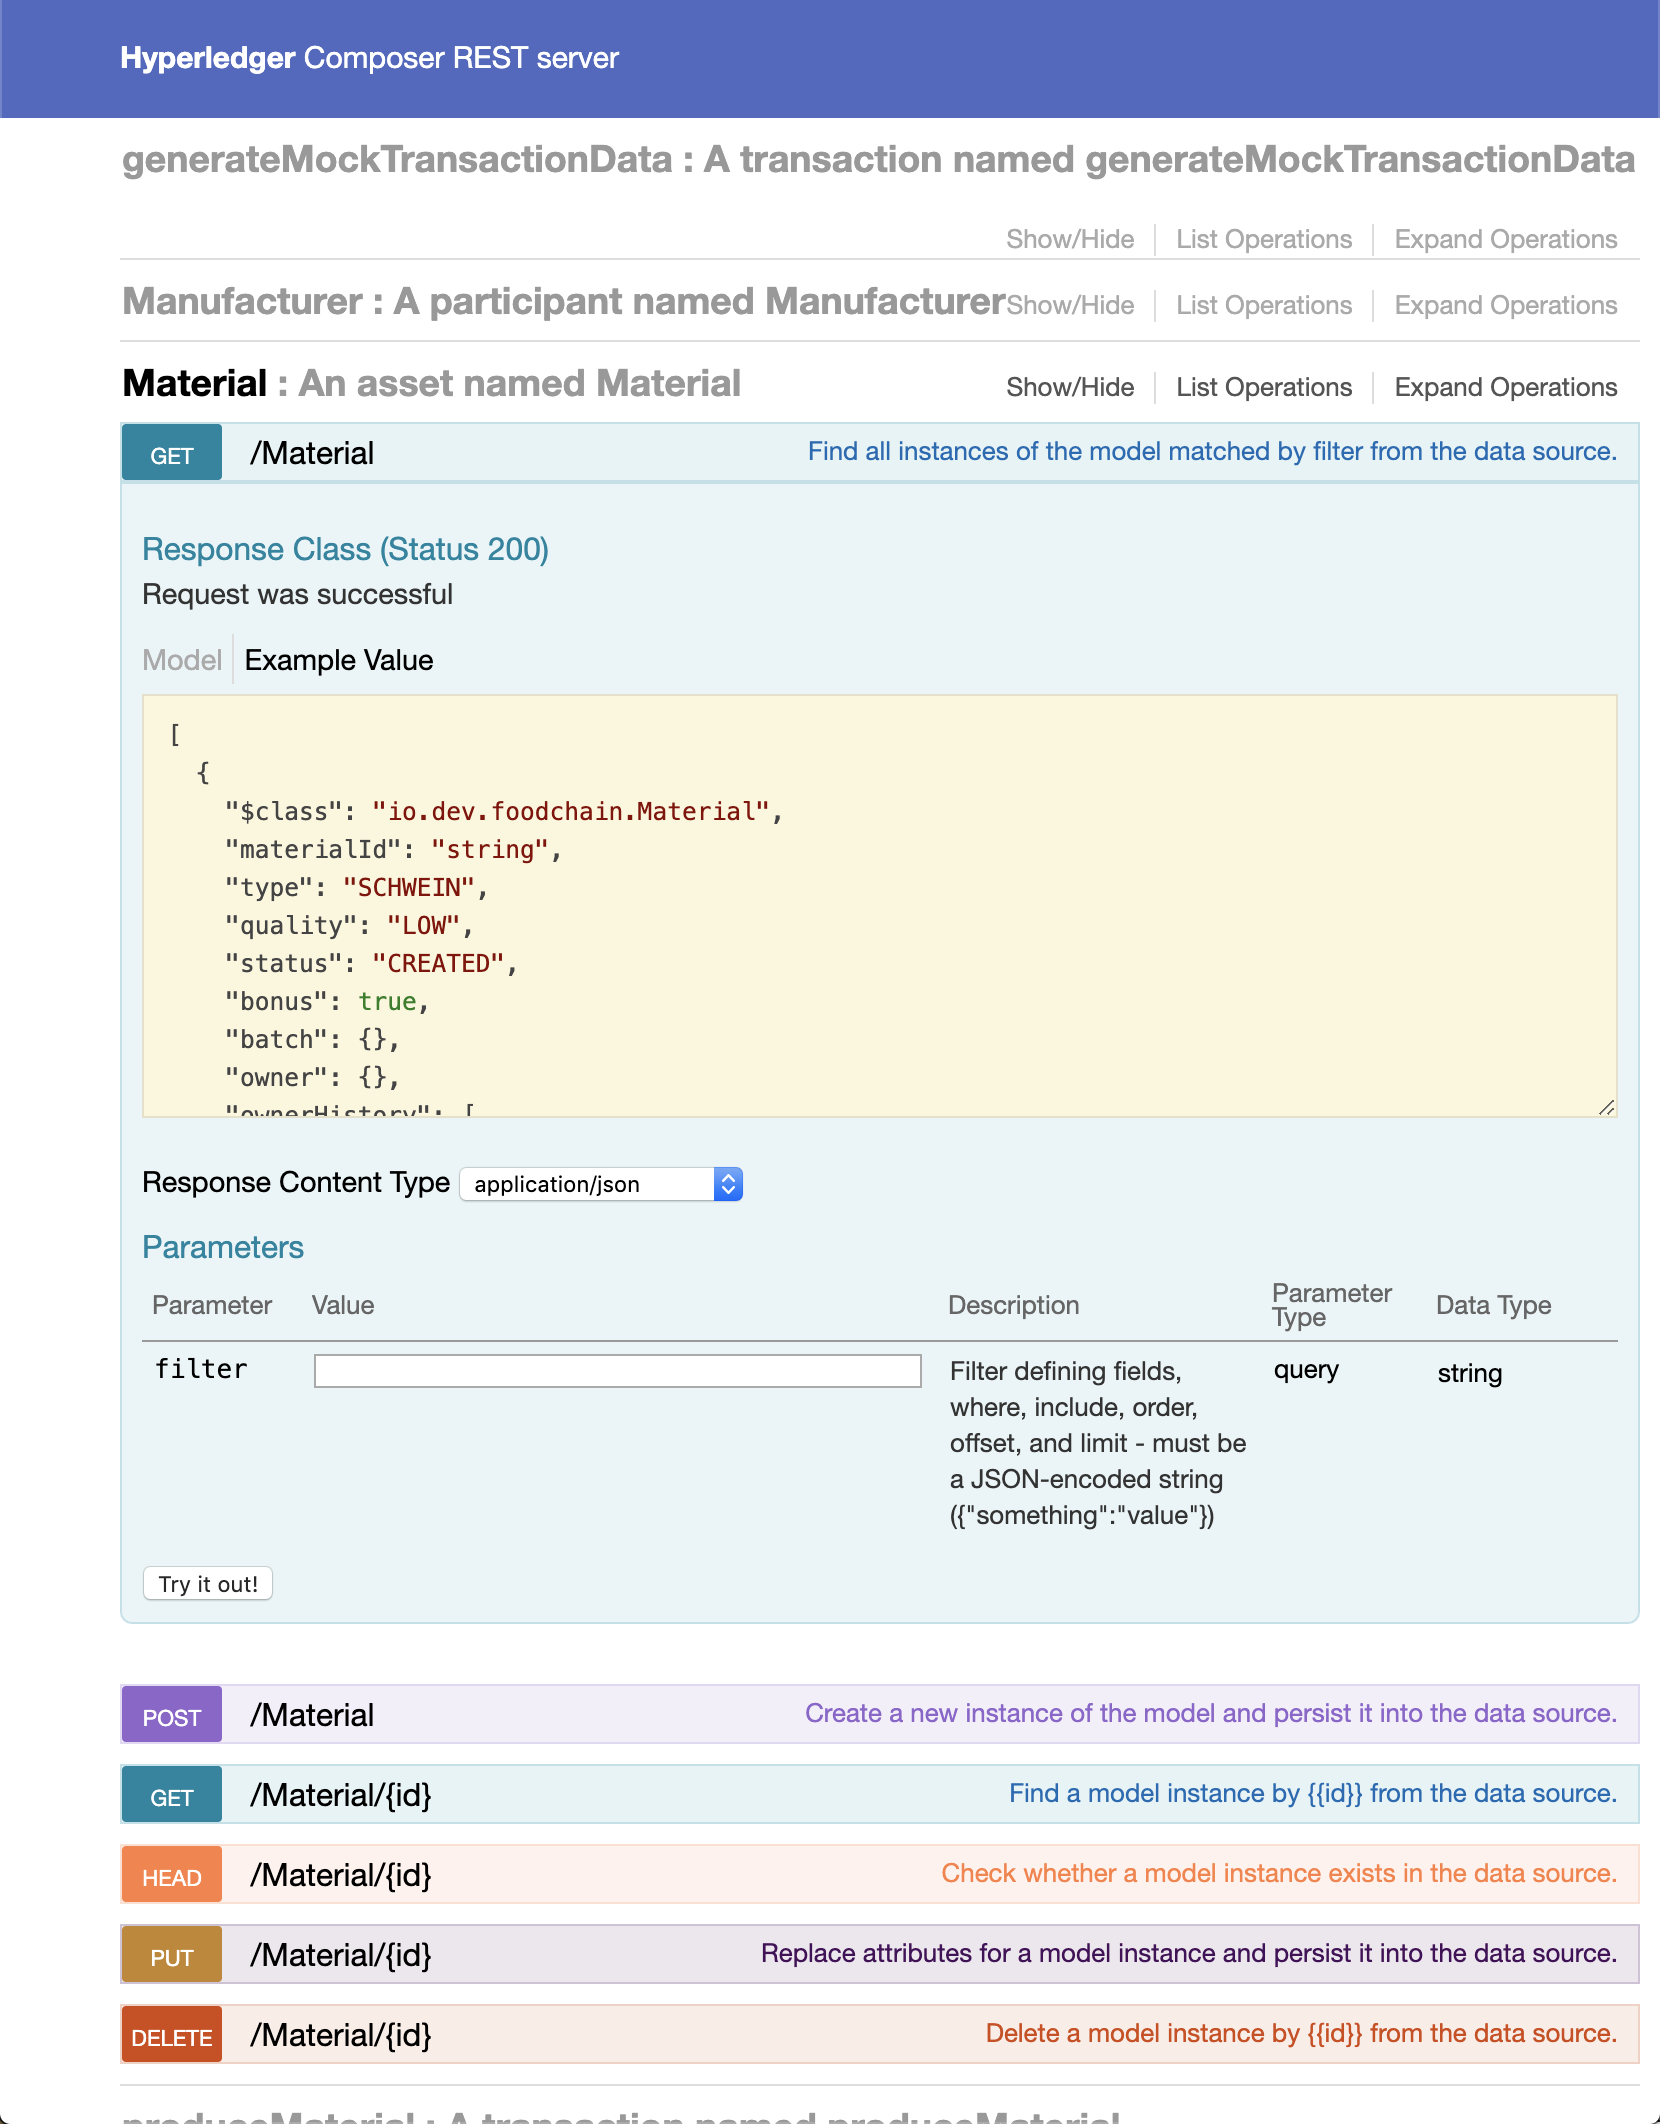
\includegraphics[width=1\linewidth]{pictures/rest-api-explorer}
	\caption[Weboberfläche der \ac{rest} \ac{api}]{Weboberfläche der \ac{rest} \ac{api}}
	\label{fig:rest-api-explorer}
\end{figure}

%3 Authentication via OAuth 2.0

\subsection{Zusammenfassung technische Umsetzung}



\newpage
